\begin{figure}[t]
    \centering
    \begin{minipage}[t]{0.49\linewidth}
        \centering
        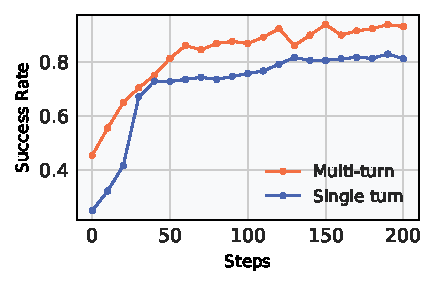
\includegraphics[width=\linewidth]{figures/compare_baseline.pdf}
        \caption{Multi-turn (5-turn) RL significantly outperforms single-turn baseline, achieving higher success rates (Pass @ 5) with similar inference cost.}
        \label{fig:compare_baseline}
    \end{minipage}
    \hfill
    \begin{minipage}[t]{0.49\linewidth}
        \centering
        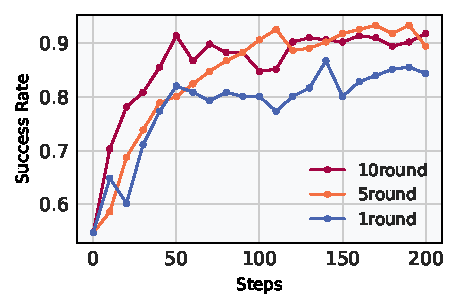
\includegraphics[width=\linewidth]{figures/multi-turn_training.pdf}
        \caption{Performance comparison when evaluating with 5 turns after training with different maximum turns (1, 5, and 10). Training with 5 turns yields the best performance, while increasing to 10 turns offers no significant gain.}
        \label{fig:1051}
        \end{minipage}
\end{figure}

\begin{figure}[t]
    \centering
    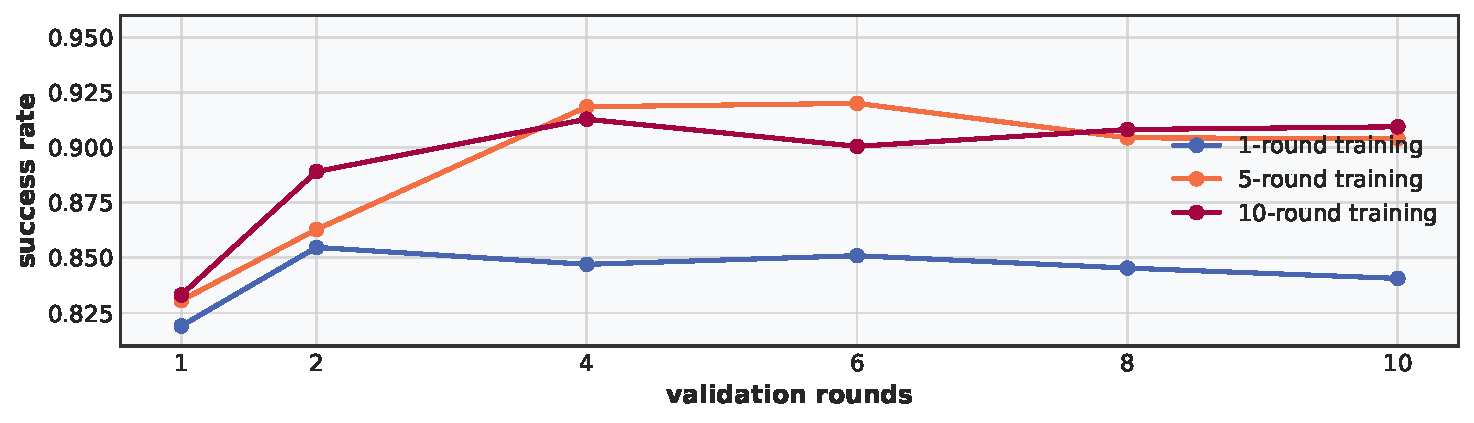
\includegraphics[width=0.98\linewidth]{figures/validation_rounds_max_checkpoint_comparison.pdf}
    \caption{\textbf{Validation performance (\texttt{Succ@k}) of models trained with different roll-out turns under varying inference-time turn budgets.} Multi-turn training (5 or 10 turns) consistently yields higher success rates across all inference turn budgets, including $k=1$, indicating better generalization even to single-turn reasoning. }
    \label{fig:validation_rounds}
    % \vspace{-0.25cm}
\end{figure}

\begin{table*}[t]
\centering
\caption{5-turn success rate across different tasks and training settings.}
\vspace{10pt}
\scriptsize 
\setlength{\tabcolsep}{2pt}
\begin{tabular}{lccccccccc}
\toprule
& \multicolumn{3}{c}{Math} & \multicolumn{2}{c}{STEM} & \multicolumn{2}{c}{QA} & \multicolumn{2}{c}{General} \\
\cmidrule(lr){2-4} \cmidrule(lr){5-6} \cmidrule(lr){7-8} \cmidrule(lr){9-10}
Model & MMQ-Math & TheoremQA & GSM8k & GPQA & MMLU-STEM & HotpotQA & ConcurrentQA & MMLU & MMLU-Pro \\
\midrule
\multicolumn{10}{l}{\textbf{Qwen2.5-1.5B-Instruct}} \\
Base Model w/o RL            & 10.9 & 11.7 & 26.6 & 21.9 & 62.5 & 2.4 & 3.1 & 52.3 & 35.2 \\
RL on MMQ-Math               & 74.8 & 20.1 & 84.7 & 22.7 & \textbf{65.5} & 19.2 & \textbf{9.5} & 43.8 & \textbf{34.8} \\
\rowcolor{gray!15}
+5turn UFO                   & \textbf{83.6} & \textbf{26.8} & \textbf{88.1} & \textbf{27.3} & 64.8 & \textbf{22.6} & \textbf{9.5} & \textbf{60.9} & \textbf{34.8} \\
\midrule
\multicolumn{10}{l}{\textbf{Qwen2.5-3B-Instruct}} \\
Base Model w/o RL            & 52.3 & 28.3 & 68.0 & 51.6 & 75.8 & 7.8 & 3.9 & 75.2 & 42.2 \\
RL on MMQ-Math               & 79.7 & 32.0 & 93.0 & 50.1 & 77.6 & 19.5 & 12.9 & 66.8 & 48.3 \\
\rowcolor{gray!15}
+5turn UFO                   & \textbf{88.5} & \textbf{40.8} & \textbf{95.3} & 52.3 & 87.5 & 26.6 & 15.2 & \textbf{85.2} & \textbf{60.9} \\
RL on HotQA                  & 72.4 & 31.8 & 89.1 & 48.4 & 81.3 & 38.3 & \textbf{16.8} & 71.5 & 49.3 \\
\rowcolor{gray!15}
+5turn UFO                   & 72.7 & 29.2 & 85.0 & \textbf{57.8} & \textbf{88.3} & \textbf{44.2} & \textbf{16.8} & 76.6 & 48.9 \\
\midrule
\multicolumn{10}{l}{\textbf{Qwen2.5-7B-Instruct}} \\
Base Model w/o RL            & 56.4 & 32.1 & 56.3 & \textbf{62.5} & 83.6 & 13.3 & 4.7 & 72.3 & 64.1 \\
RL on MMQ-Math               & 85.1 & 33.6 & 95.2 & 50.8 & \textbf{84.8} & 26.3 & 14.1 & 73.4 & 52.3 \\
\rowcolor{gray!15}
+5turn UFO                   & \textbf{93.0} & \textbf{42.1} & \textbf{96.8} & 56.9 & \textbf{84.8} & \textbf{28.6} & \textbf{16.4} & \textbf{80.5} & \textbf{58.8} \\
\midrule
\multicolumn{10}{l}{\textbf{Llama3.2-1B-Instruct}} \\
Base Model w/o RL*           & 2.3 & 2.3 & 1.6 & 1.6 & 4.6 & 0.8 & 0.8 & 3.9 & 2.3 \\
RL on MMQ-Math               & 53.9 & 21.1 & 52.3 & 20.3 & 57.0 & 19.5 & 0.8 & 57.8 & \textbf{32.8} \\
\rowcolor{gray!15}
+5turn UFO                   & \textbf{64.8} & \textbf{26.8} & \textbf{56.3} & \textbf{26.6} & \textbf{60.2} & \textbf{21.1} & \textbf{1.6} & \textbf{66.4} & \textbf{32.8} \\
\midrule
\multicolumn{10}{l}{\textbf{Llama3.2-3B-Instruct}} \\
Base Model w/o RL            & 50.8 & 20.3 & 48.4 & 47.7 & 77.3 & 29.7 & 6.0 & 65.6 & 49.2 \\
RL on MMQ-Math               & 86.7 & 24.2 & 92.2 & 46.9 & 78.1 & \textbf{44.5} & 13.3 & 71.1 & 60.9 \\
\rowcolor{gray!15}
+5turn UFO                   & \textbf{92.2} & \textbf{32.0} & \textbf{93.8} & \textbf{50.8} & \textbf{82.0} & 39.8 & \textbf{14.8} & \textbf{82.8} & \textbf{66.4} \\
\bottomrule
\end{tabular}
\label{tab:5turn-success}
\end{table*}

\begin{figure}[t]
    \centering
    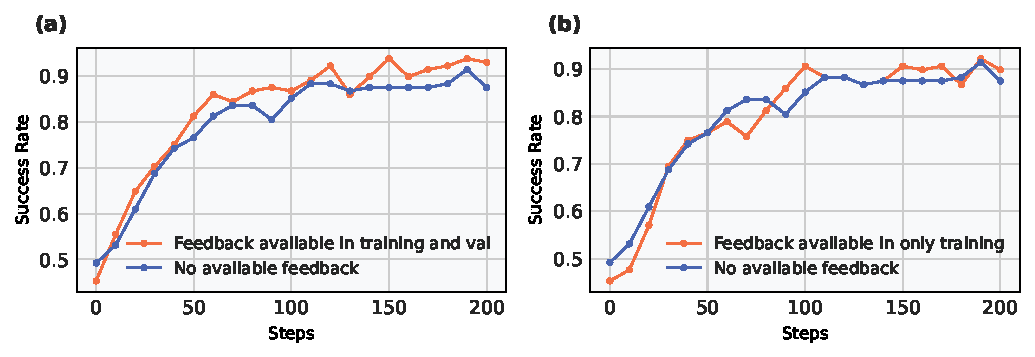
\includegraphics[width=0.98\linewidth]{figures/feedback_comparisons_side_by_side.pdf}
    \caption{\textbf{Comparison of success rate with multi-turn setting.} (a) with feedback prompt in both training and validation compared to blank prompt; (b) with feedback prompt only in training compared to blank prompt.}
    \label{fig:compare}
    % \vspace{-0.25cm}
\end{figure}

\subsection{Experimental Results and Findings}
\linespread{0.97}\selectfont
In this section, we present empirical findings that address three central questions in our study of multi-turn reinforcement learning with unary feedback:

\begin{enumerate}[noitemsep, topsep=0pt, leftmargin=*]
    \item Section~\ref{sec:4.2.1}: Does multi-turn RL unlock stronger reasoning than single-turn training?
    \item Section~\ref{sec:4.2.2}: Can models effectively revise their answers from sparse feedback alone?
    \item Section~\ref{sec:4.2.3}: How do reward shaping strategies impact reasoning efficiency and diversity?
\end{enumerate}

We explore each question in the following subsections, with quantitative analyses and ablation studies. Additional qualitative examples and robustness checks are included in the Appendix.


\subsubsection{Multi-turn RL Unlocks Higher Upper Bound of LLM Reasoning}


\label{sec:4.2.1} 
We compare models trained with multi-turn RL against single-turn PPO baselines, using \texttt{Succ@5} on a held-out validation set evaluated at 21 checkpoints across 200 training steps. During validation, each agent is allowed up to 5 interaction turns per problem ($k=5$). 

As shown in Figure~\ref{fig:compare_baseline}, multi-turn training consistently outperforms the single-turn baseline, \textbf{achieving up to 14\% higher success rate} with comparable inference cost. This highlights the benefit of iterative revision under sparse feedback.

Furthermore, we conduct additional experiments comparing various multi-turn training budgets ($T_{\text{max}} = 1, 5, 10$) while consistently using a 5-turn validation setup. Findings presented in Figure~\ref{fig:1051} demonstrate that larger training budgets yield enhanced performance relative to the single-turn baseline. Notably, both the $T_{\text{max}}=10$ and $T_{\text{max}}=5$ configurations deliver \textbf{more than a 6\% relative improvement} over single-turn training at their peak, clearly emphasizing the benefits of multi-turn training.



To validate the robustness of these improvements, we expand our analysis by evaluating peak-performing models trained with $T_{\text{max}} \in \{1, 5, 10\}$ across varied inference-time interaction budgets ($k \in \{1, 2, 4, 6, 8, 10\}$). The results illustrated in Figure~\ref{fig:validation_rounds} reinforce previous observations, consistently showing superior Succ@$k$ performance by models trained under multi-turn conditions. Intriguingly, these improvements are observable even at the lowest inference budget ($k=1$), suggesting that multi-turn training enhances not only iterative performance but also generalizes well to single-shot scenarios. 

\begin{figure}[t]
    \centering
    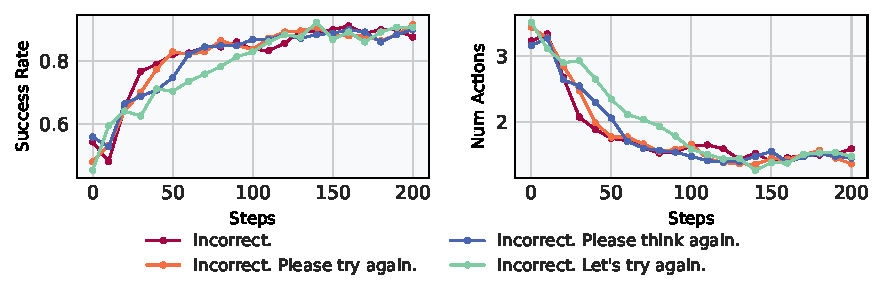
\includegraphics[width=0.9\linewidth]{figures/prompt_strategies_comparison.pdf}
    \caption{\textbf{Validation under different verbal feedback prompts.} Success rates and action counts remain consistent across all variants, demonstrating UFO's robustness to various prompts.}
    \label{fig:prompt}
    % \vspace{-0.25cm}
\end{figure}

\begin{figure}[t]
    \centering
    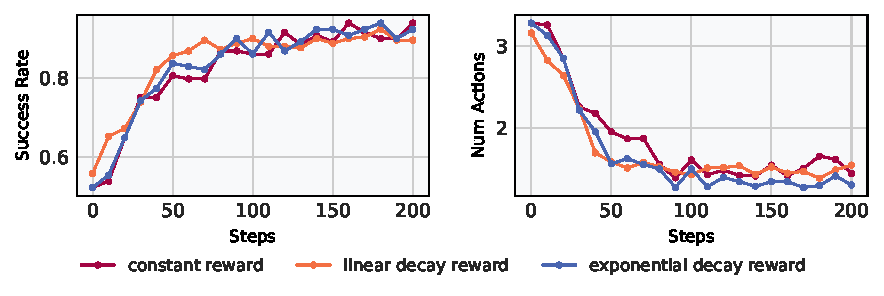
\includegraphics[width=0.9\linewidth]{figures/reward_decay_comparison.pdf}
    \caption{\textbf{Comparison of reward shaping strategies.} While constant, linear decay, and exponential decay schedules achieve similar success rates (left), exponential decay consistently leads to fewer actions per episode (right), indicating more efficient problem solving with less external supervision.}
    \label{fig:reward_design}
    % \vspace{-0.25cm}
\end{figure}

Table~\ref{tab:5turn-success} summarizes three key findings across five models and nine datasets. First, applying 5-turn UFO consistently improves performance over single-turn RL on the same task, confirming its in-domain effectiveness. Second, UFO-trained models generalize reliably to new domains, with consistent gains observed across four broad categories: math, STEM, QA, and general knowledge. Third, math-trained models tend to generalize more strongly than QA-trained ones, possibly due to the more structured and logically consistent nature of mathematical reasoning. %Note that MMLU is a four-way multiple-choice benchmark, and we allow the model to make up to five independent attempts per question. Under this setting, the model is theoretically guaranteed to select the correct answer within five trials. Nevertheless, we adopt this setting to ensure consistency with prior work and to allow fair comparison across different datasets.
These trends hold across two families of open-source models, Qwen2.5 and Llama3.2, spanning from 1B to 7B in scale, suggesting the effectiveness of UFO are robust to both model architecture and size. \textit{We note that LLaMA3-1B shows relatively lower base performance compared to official numbers, possibly due to format-following issues.}

These trends suggest that by enabling models to explore alternative reasoning paths and revise prior failures based on sparse feedback, UFO provides a principled path toward robust multi-turn and cross-task generalization.

\subsubsection{Multi-turn Setting Enables LRMs to Revise From Feedback}
\label{sec:4.2.2}

The multi-turn setting enables agents to engage repeatedly with each prompt (up to $T_{\text{max}}$ turns), thereby constructing richer and more informative interaction trajectories from the same training data. This enhanced utilization of feedback is hypothesized to extract more meaningful learning signals per problem, potentially improving solution quality and accelerating convergence, especially in data-limited contexts.

To empirically validate that LRMs can be improved effectively utilizing conversational feedback for revision, we compare 5-turn training scenarios with and without explicit feedback prompts. Results presented in Figure~\ref{fig:compare}(a) support this hypothesis, \textbf{demonstrating an over 8\% peak performance improvement when explicit feedback is provided.}

An additional analysis with feedback prompt only in training (Figure~\ref{fig:compare}(b)) reveals performance improvement as well. This suggests that multi-turn training can even intrinsically enhance model reasoning capabilities.

Finally, our robustness analysis in the Figure~\ref{fig:prompt} shows that the effectiveness of this approach is preserved across a range of prompt formulations, underscoring its practical applicability in real-world scenarios.

\subsubsection{Reward Shaping Encourages Efficient Problem Solving}
\label{sec:analysis_reward_decay}
\label{sec:4.2.3}

We investigate how different reward schedules influence the agent's learning behavior, particularly in encouraging early success versus allowing extended exploration. All schedules define a reward $r(n)$ based on the turn index $n$ when the first correct answer is produced, with $n \in \{1, \dots, T_{\text{max}}\}$.

We define and evaluate three distinct reward schedules. Following the formulas proposed in Section~\ref{sec:reward_design}, we compare three approaches: (1) \textbf{Exponential Decay:} $r_{\text{exp}}(n) = \gamma^n$ (with $\gamma=0.5$), (2) \textbf{Linear Decay:} $r_{\text{lin}}(n) = \max(0, 1 - 0.2(n-1))$, (3) \textbf{Constant Reward:} $r_{\text{const}}(n) = 1.$
All schedules operate for $n \in {1, \dots, T_{\text{max}}}$.
The agent's objective remains to maximize the expected cumulative reward.

Experimental validation (Figure~\ref{fig:reward_design}) confirms that \textbf{exponential reward decay notably reduces the mean number of actions by roughly 10\%}, without sacrificing overall success rates. This reduction in action count suggests that the exponential decay schedule encourages the model to engage in more profound self-reflection and systematic thinking before generating a response.

Considering the normalized penalty term in our experiment (Equation~\ref{eq:penalty}),
we count the number of non-repetitive answer for each validation round, as shown in Figure~\ref{fig:non-repetitive}. The percentage \textbf{increases from 80\% to over 90\%}, suggesting that the model performs better in the later stages of training as the model learned to explore and self-reflect.


\begin{figure}[!th]
    \centering
    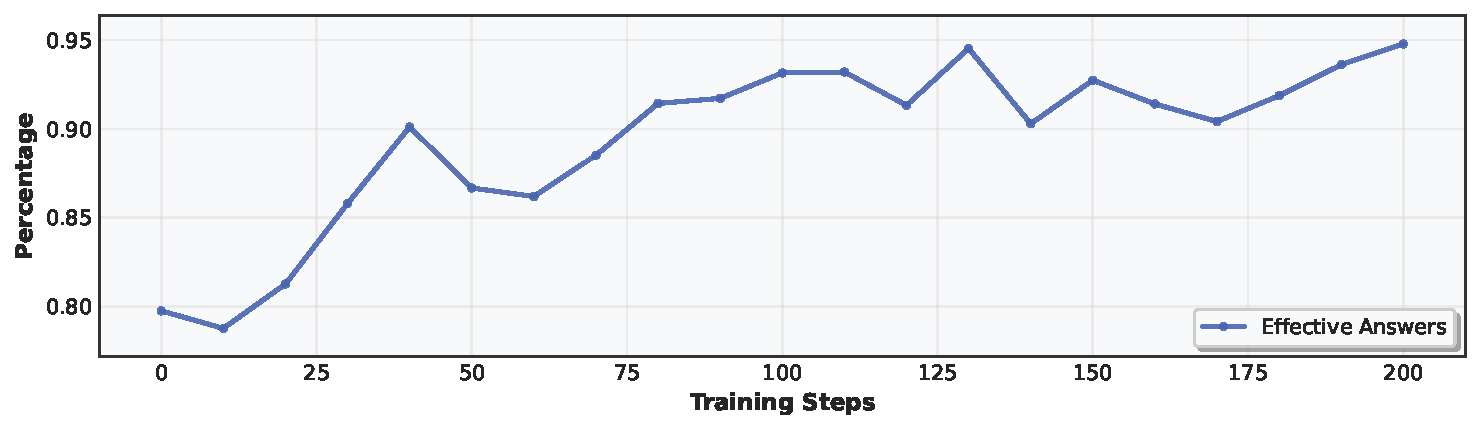
\includegraphics[width=0.98\linewidth]{figures/nonrepetitive_answers.pdf}
    \caption{\textbf{Proportion of effective answers over training.} The upward trend suggests improved diversity across turns, which reduces penalty from repeated responses and contributes to higher overall rewards.}
    \label{fig:non-repetitive}
    % \vspace{-0.25cm}
\end{figure}
